\documentclass{article}
\usepackage{amsmath}
\usepackage{graphicx}
\usepackage{hyperref}
\usepackage{geometry}
\usepackage[section]{placeins}
\geometry{a4paper, margin=1in}

\title{Analysis of Crime in Chicago (2013-2023)}
\author{Xinyi Zhu}
\date{\today}

\begin{document}

\maketitle

\section{Introduction}

Crime analysis is a critical component of urban safety and public policy planning. This report focuses on crime data from Chicago over an eleven-year period, from 2013 to 2023. The primary objectives of this analysis are as follows:
\begin{itemize}
    \item To assess the yearly number of crimes reported in Chicago.
    \item To calculate and analyze the average accumulated crime cases per year.
    \item To categorize and analyze the types of crimes committed.
    \item To investigate the geographical distribution of crimes within the city.
\end{itemize}

Understanding the temporal and spatial distribution of crimes can provide valuable insights into underlying patterns and trends. Such information is crucial for law enforcement agencies, policy makers, and community organizations to devise effective crime prevention strategies and allocate resources efficiently.

\section{Yearly Number of Crimes (2013-2023)}


\begin{figure}
    \centering
    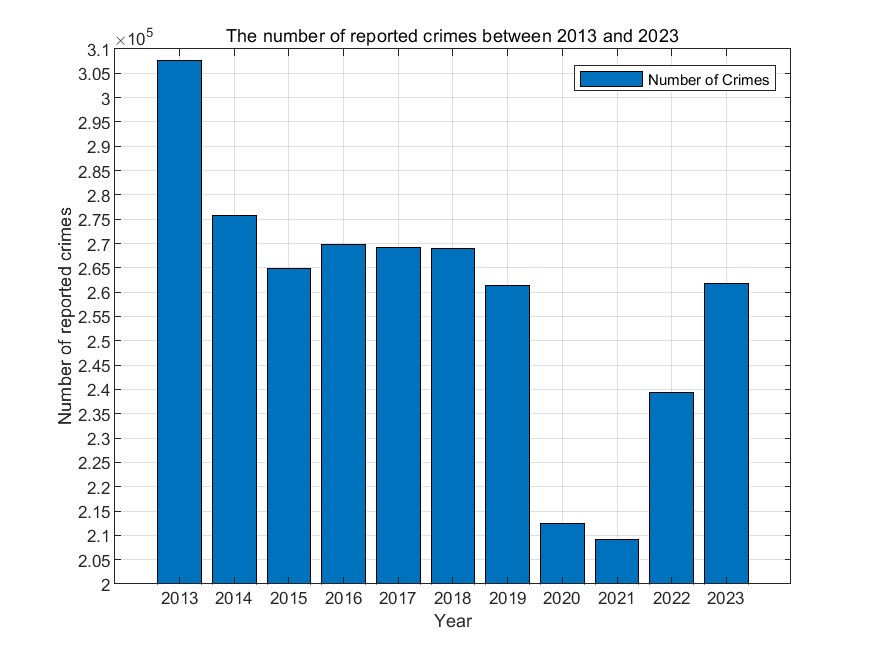
\includegraphics[width=0.8\linewidth]{Yearly_crimeNumber_bar.jpg}
    \caption{The number of reported crimes between 2013 and 2023}
    \label{fig:yearly_crimes}
\end{figure}

   \begin{itemize}
    \item Since 2014, the number of crime cases has significantly reduced, with only around 270,000 reported crimes in 2014 and even lower for the following years, which is a sharp reduction from over 300,000 reported incidents in 2013.
    \item An evident reduction in the number of crime cases in 2020 and 2021 due to the COVID-19 pandemic lockdown.
    \item A subsequent rise in crime reports in 2022 and 2023, suggesting a recent upward trend in criminal activities since the pandemic situation eased and lockdowns gradually stopped.
\end{itemize}
\FloatBarrier

\section{Average Accumulated Crime Cases in a Year}


\begin{figure}[h!]
    \centering
    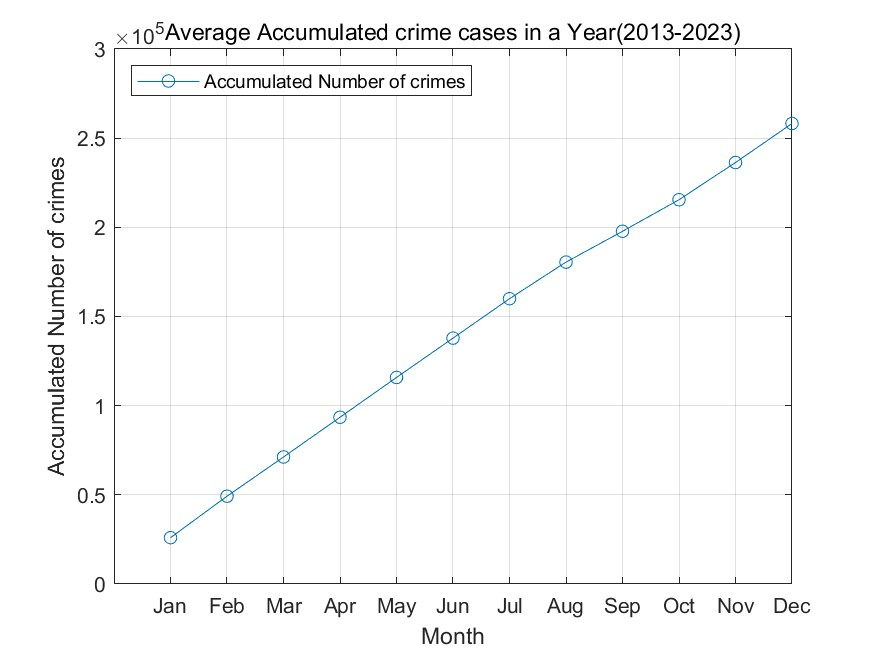
\includegraphics[width=0.8\linewidth]{Accumulated_crimeNumber_line.jpg}
    \caption{Average accumulated number of crimes in a year (2013-2023)}
    \label{fig:accumulated_crimes}
\end{figure}

Figure \ref{fig:accumulated_crimes} illustrates the average accumulated number of crimes per month over the eleven-year period. The linear trend observed suggests a consistent accumulation of crime cases throughout the year, with no significant deviations in monthly crime accumulation patterns, only a slight dip around August. This steady increase highlights the ongoing challenge of crime prevention and the need for continuous efforts to address criminal activities.
\FloatBarrier

\section{Predicted Accumulated Crime Numbers for 2023 and 2024}

\begin{figure}[h!]
    \centering
    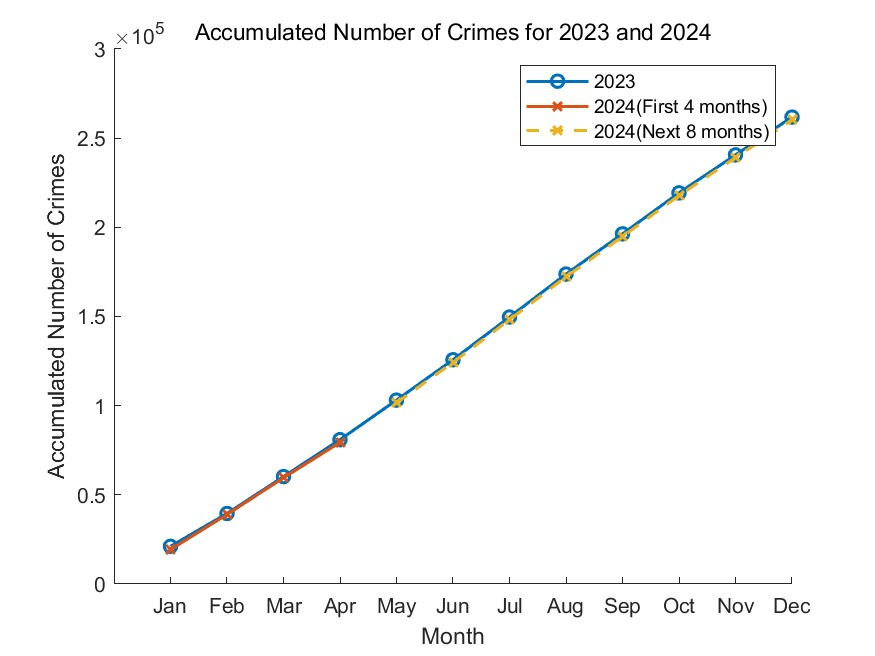
\includegraphics[width=0.8\textwidth]{Predicted_accumulated_crimeNumber_line.jpg}
    \caption{Accumulated number of crimes for 2023 and 2024 (predicted)}
    \label{fig:predicted_crimes}
\end{figure}

Figure \ref{fig:predicted_crimes} compares the accumulated number of crimes for 2023 and the first four months of 2024, with projections for the remainder of 2024. The projection suggests similar crime trends continuing into 2024, with a slight increase compared to 2023. This predictive analysis can assist in proactive crime prevention measures and resource allocation.
\FloatBarrier

\section{Analysis of Crime Types}

\begin{figure}[h!]
    \centering
    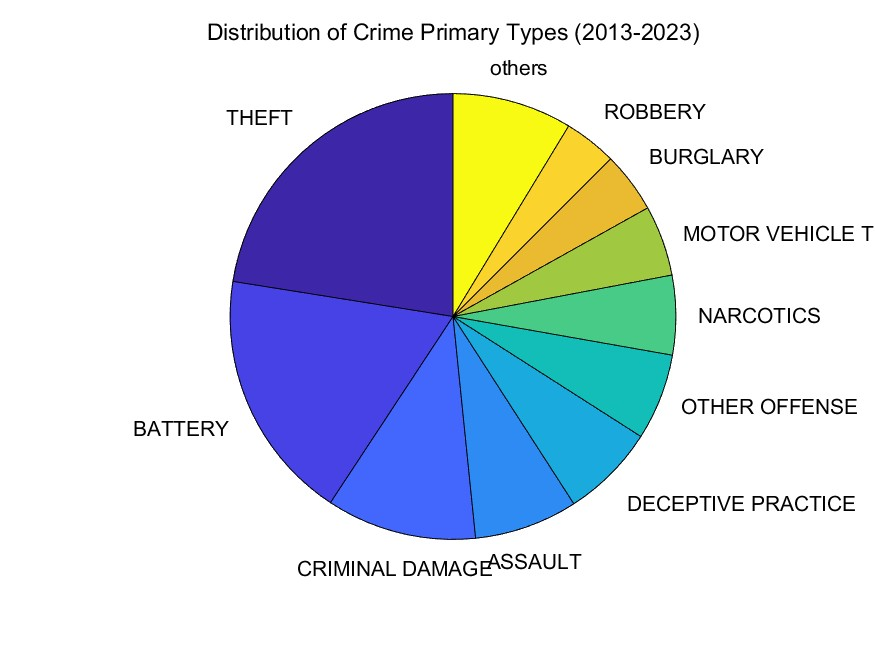
\includegraphics[width=0.8\textwidth]{Crime_type_pie.jpg}
    \caption{Distribution of crime primary types (2013-2023)}
    \label{fig:crime_types}
\end{figure}


The pie chart in Figure \ref{fig:crime_types} presents the distribution of primary crime types reported between 2013 and 2023. Theft is the most prevalent crime, comprising significant portions of the total, followed by battery and assault. Other prevalent crime types include Assault, Criminal Damage, and Narcotics-related offenses. Lesser, but still notable, are crimes like Burglary, Motor Vehicle Theft, and Deceptive Practices. Understanding the distribution of crime types is essential for developing targeted intervention strategies and allocating resources effectively to combat specific types of crimes.

\FloatBarrier
\section{Crime Descriptions Analysis}

\begin{figure}[h!]
    \centering
    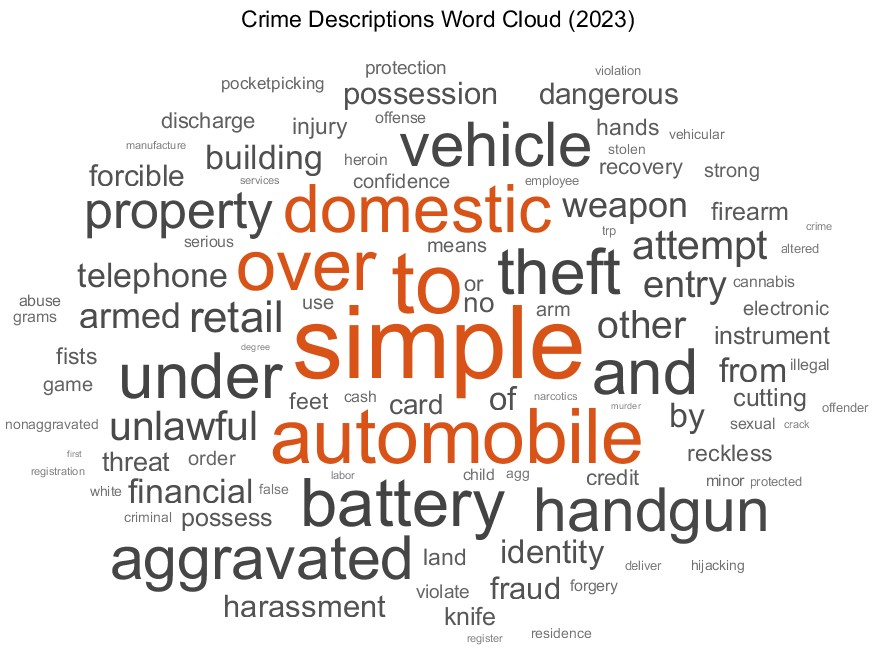
\includegraphics[width=0.8\textwidth]{Crime_description_wordcloud.jpg}
    \caption{Crime descriptions word cloud (2023)}
    \label{fig:crime_wordcloud}
\end{figure}

The word cloud in Figure \ref{fig:crime_wordcloud} provides a visual representation of the most common terms found in crime descriptions for the year 2023. Terms like "domestic," "simple," "battery," and "automobile" appear prominently, indicating their frequent occurrence in crime reports. 

The term "domestic" often refers to domestic violence or disputes, which remains a significant issue. Studies indicate that domestic violence incidents can spike due to economic stress or isolation, factors that have been particularly relevant during the pandemic.

"Simple" usually refers to simple assault, a less severe form of assault that doesn't involve a weapon or result in serious injury. Simple assaults are among the most commonly reported violent crimes in urban areas.

The prevalence of the term "battery" suggests a high incidence of physical altercations. Research shows that battery cases often correlate with alcohol consumption and high-stress environments.

The term "automobile" points to the frequent occurrence of vehicle-related crimes, such as theft or vandalism. Automobile-related crimes are common in metropolitan areas due to the high density of vehicles.

This qualitative analysis offers insights into the nature of crimes and can guide the development of specific crime prevention programs.

\FloatBarrier

\section{Crime Location Analysis}

\begin{figure}[h!]
    \centering
    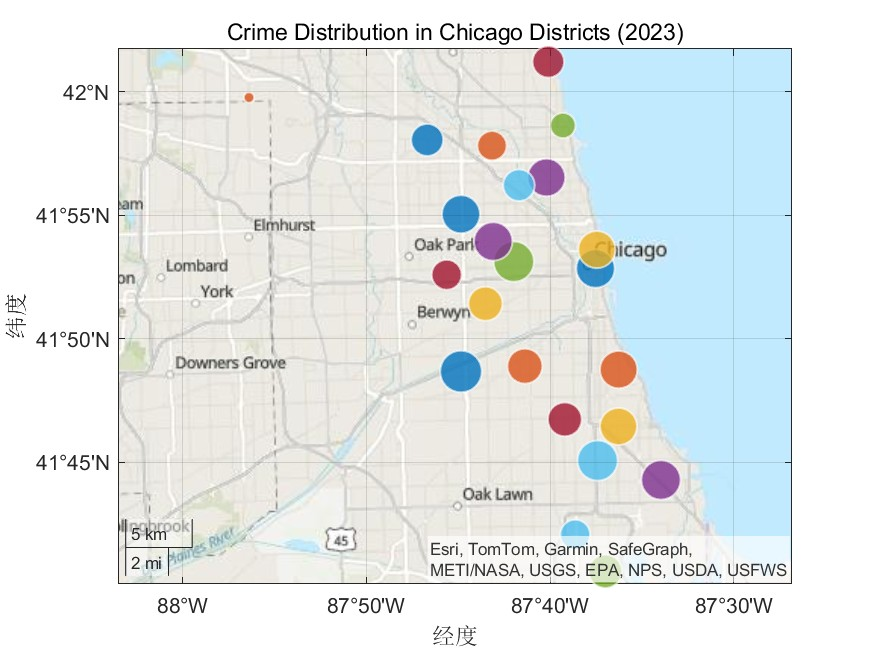
\includegraphics[width=0.8\textwidth]{Crime_distribution_bubble.jpg}
    \caption{Crime distribution in Chicago districts (2023)}
    \label{fig:crime_distribution}
\end{figure}

Figure \ref{fig:crime_distribution} shows the spatial distribution of crimes across various districts in Chicago for the year 2023. The bubble chart highlights certain districts as hotspots for criminal activities, indicating a higher concentration of reported crimes. This geographical analysis helps identify areas that require increased policing efforts and community support to mitigate crime rates.




\end{document}
